\documentclass[10pt,a4paper]{article}

% ===== Fonts (xelatex) =====
\usepackage{fontspec}
\defaultfontfeatures{Ligatures=TeX}
\newcommand{\tgpath}{/usr/local/texlive/2022/texmf-dist/fonts/opentype/public/tex-gyre/}
\setmainfont[
  Path           = \tgpath,
  Extension      = .otf,
  UprightFont    = texgyrepagella-regular,
  BoldFont       = texgyrepagella-bold,
  ItalicFont     = texgyrepagella-italic,
  BoldItalicFont = texgyrepagella-bolditalic,
]{TeX Gyre Pagella}
\setsansfont[
  Path           = \tgpath,
  Extension      = .otf,
  Scale          = 0.94,
  UprightFont    = texgyreheros-regular,
  BoldFont       = texgyreheros-bold,
  ItalicFont     = texgyreheros-italic,
  BoldItalicFont = texgyreheros-bolditalic,
]{TeX Gyre Heros}
\setmonofont[
  Path           = \tgpath,
  Extension      = .otf,
  Scale          = 0.88,
  UprightFont    = texgyrecursor-regular,
  BoldFont       = texgyrecursor-bold,
  ItalicFont     = texgyrecursor-italic,
  BoldItalicFont = texgyrecursor-bolditalic,
]{TeX Gyre Cursor}

% ===== Page layout =====
\usepackage[a4paper, top=1.7cm, bottom=1.8cm, left=2.1cm, right=2.1cm]{geometry}
\usepackage{microtype}

% ===== Color palette =====
\usepackage[dvipsnames,table]{xcolor}
\definecolor{primary}{HTML}{1F3A5F}    % deep navy
\definecolor{accent}{HTML}{0E7C86}     % teal
\definecolor{softgray}{HTML}{F4F5F7}
\definecolor{rulegray}{HTML}{C5CAD1}
\definecolor{mutedtext}{HTML}{4A5568}
\definecolor{warm}{HTML}{C2410C}

% ===== Core packages =====
\usepackage{url}
\usepackage{amsmath,amssymb}
\usepackage{graphicx}
\usepackage{float}
\usepackage{needspace}
\usepackage{subcaption}
\usepackage{booktabs}
\usepackage{tikz}
\usepackage{enumitem}
\usepackage{titling}
\usepackage{titlesec}
\usepackage{authblk}
\usepackage{caption}
\usepackage[most]{tcolorbox}
\usepackage{fancyhdr}
\usepackage{hyperref}
\usetikzlibrary{arrows.meta, positioning, shapes.geometric, fit, backgrounds, calc, shadows.blur}

% ===== Spacing & lists =====
\linespread{1.05}
\setlength{\parskip}{2pt}
\setlength{\parindent}{0pt}
\setlength{\floatsep}{5pt plus 1pt minus 1pt}
\setlength{\textfloatsep}{6pt plus 1pt minus 2pt}
\setlength{\intextsep}{5pt plus 1pt minus 1pt}
\renewcommand{\arraystretch}{0.95}
\renewcommand{\figurename}{Fig.}

\setlist[itemize]{leftmargin=1.3em, itemsep=1.5pt, parsep=0pt, topsep=2pt,
                  label={\color{accent}\footnotesize$\blacktriangleright$}}
\setlist[enumerate]{leftmargin=1.6em, itemsep=1.5pt, parsep=0pt, topsep=2pt,
                    label={\color{primary}\sffamily\bfseries\arabic*.}}

% ===== Section headings: colored number-box + thin rule =====
\titleformat{\section}[hang]
  {\sffamily\large\bfseries\color{primary}}
  {\colorbox{primary}{\color{white}\sffamily\bfseries\,\thesection\,}\hspace{0.6em}}
  {0pt}{}
  [\vspace{1pt}{\color{rulegray}\rule{\linewidth}{0.4pt}}]
\titleformat{\subsection}[runin]
  {\sffamily\small\bfseries\color{accent}}
  {\thesubsection}{0.5em}{}[.\ ]
\titlespacing{\section}{0pt}{9pt plus 2pt minus 1pt}{4pt}
\titlespacing{\subsection}{0pt}{4pt}{0.4em}

% ===== Caption styling =====
\captionsetup{font=small, labelfont={sf,bf,color=primary}, labelsep=period,
              skip=3pt, justification=justified}
\captionsetup[sub]{font=footnotesize, labelfont={sf,bf,color=accent}, labelsep=period, skip=2pt}

% ===== Abstract / keywords box =====
\newtcolorbox{infobox}{
  enhanced, colback=softgray, colframe=rulegray, boxrule=0.3pt,
  arc=2pt, left=8pt, right=8pt, top=5pt, bottom=5pt,
  before skip=2pt, after skip=4pt,
  borderline west={2.2pt}{0pt}{accent},
}

% ===== URLs / hyperlinks =====
\hypersetup{colorlinks=true, urlcolor=accent, linkcolor=primary, citecolor=primary,
            breaklinks=true}
\sloppy
\emergencystretch=1.5em

% ===== Page footer =====
\pagestyle{fancy}
\fancyhf{}
\renewcommand{\headrulewidth}{0pt}
\renewcommand{\footrulewidth}{0pt}
\fancyfoot[L]{\scriptsize\sffamily\color{mutedtext}Context-Aware Emotional TTS\,\textbullet\,MAIE5531 Milestone}
\fancyfoot[R]{\scriptsize\sffamily\color{mutedtext}\thepage\ / \pageref*{LastPage}}
\usepackage{lastpage}

% ===== Title block =====
\setlength{\droptitle}{-2em}
\pretitle{\begin{center}\sffamily\bfseries\Large\color{primary}}
\posttitle{\par\end{center}\vspace{-0.8em}}
\preauthor{\begin{center}\sffamily\small\color{mutedtext}}
\postauthor{\end{center}\vspace{-1.5em}}
\predate{}\postdate{}\date{}
\renewcommand\Affilfont{\sffamily\scriptsize\itshape\color{mutedtext}}
\setcounter{secnumdepth}{3}

\title{Context-Aware Emotional TTS for Game AI Dubbing\\[2pt]
  {\normalsize\sffamily\mdseries\itshape\color{mutedtext}%
   Milestone Report\,\textbullet\,MAIE5531 GenAI and LLM\,\textbullet\,April 2026}}
\author[1]{HE Yunlin}
\author[1]{WANG Yifu}
\author[1]{SU Ziyao}
\author[1]{HAN Shipeng}
\affil[1]{AI \& Entrepreneurship, Hong Kong University of Science and Technology}

\begin{document}
\maketitle
\thispagestyle{fancy}

\vspace{-0.8em}
\begin{infobox}
\noindent\small
{\sffamily\bfseries\color{primary}Abstract.}~We extend our Phase-1 Qwen3-TTS 1.7B voice cloner (SIM\textsubscript{gt}=0.689, RTF=0.357) with an \emph{Emotional-Aware Context} layer: scene + dialogue $\rightarrow$ character-RAG $\rightarrow$ LLM structured emotion annotations $\rightarrow$ emotion-arc tracking $\rightarrow$ dispatch to the best of eight TTS backends with emotion-matched reference audio. A FastAPI service + React/Recharts front end close the loop. Remaining work: three-way comparative evaluation and a subjective MOS study, targeted for May~10,~2026.\\[2pt]
{\sffamily\bfseries\color{primary}Keywords.}~Emotional TTS~\textbullet~Voice Cloning~\textbullet~Retrieval-Augmented Generation~\textbullet~LLM~\textbullet~Game AI
\end{infobox}

\vspace{2pt}

%% ============================================================
\section{Introduction \& Problem Recap}
%% ============================================================
Phase~1 \emph{solved} the timbre side of character cloning: on an 18-sentence test set, our Qwen3-TTS 1.7B SFT reached \textbf{SIM\_gt = 0.689} and \textbf{WER = 4.25\%} at \textbf{RTF = 0.357} via CUDA-Graph capture --- a $7.1\times$ speed-up over native decoding on an A100 (\texttt{docs/report/report.pdf}). The cloned voice reliably \emph{sounds} like the character but sounds the same in every scene --- consolation, teasing, cold confrontation all share one baseline prosody. Narrative-driven games need scene-aware emotion, and manually tagging every line is exactly what a voice-actor pipeline should avoid. This milestone replaces the human director with an automated one driven by an LLM, RAG, and an emotion-arc tracker.

%% ============================================================
\section{Completed Work}
%% ============================================================
\textbf{Phase~1 recap.} We collected 664 clips ($\sim$28\,min) of one game character via a Bilibili~$\rightarrow$~source-separation~$\rightarrow$~diarization~$\rightarrow$~VAD~$\rightarrow$~ASR pipeline, fine-tuned Qwen3-TTS 1.7B (v5, ep.~3), and benchmarked against Fish S2 Pro. The \texttt{FasterQwen3TTS} CUDA-Graph wrapper brought RTF from $2.54$ to $0.357$ with no quality loss (Fig.~\ref{fig:phase1}b). A bf16 speaker-embedding accumulation bug, fixed by an fp32 running sum, recovered SIM\_gt \textbf{+141\%} (0.29~$\rightarrow$~0.69), documented in Phase~1's \texttt{README.md}~§14.

\textbf{Phase~2 --- Emotional-Aware Context system (this milestone).} All new modules live under \texttt{src/} and plug into a single FastAPI service + React front end.
\begin{itemize}
  \item \textbf{LLM Context Engine} (\texttt{context\_engine/}): system prompt + 4 few-shot exemplars force GPT-4o to emit a strict Pydantic \texttt{EmotionAnnotation}\,=\,\{\texttt{emotion, intensity, pace, style, ref\_emotion\_category, fish\_audio\_tags}\}; \texttt{ref\_emotion\_category} is constrained to one of six buckets the dispatcher can act on.
  \item \textbf{Character RAG} (\texttt{rag/}): four Markdown files under \texttt{data/character\_kb/} (\texttt{personality, relationships, emotional\_patterns, catchphrases}) are chunked, embedded with \texttt{BAAI/bge-large-zh-v1.5}, stored in a local ChromaDB; top-$k$ hits are injected into every prompt so emotions stay in character.
  \item \textbf{Emotion Arc Tracker} (\texttt{emotion\_tracker/}): a 10-turn sliding window + a hand-crafted transition-distance table flags abrupt jumps and feeds the last $N$ states back into the LLM prompt so consecutive lines form a coherent arc.
  \item \textbf{Emotion-aware reference selection.} The 664 clips are classified into six buckets (\emph{tender, calm, playful, intense, cold, intimate}); the 5 highest-confidence per bucket are distilled into \texttt{data/emotion\_buckets.json} (Fig.~\ref{fig:phase1}a) and looked up at inference time.
  \item \textbf{Multi-backend TTS dispatcher} (\texttt{tts/}): 8 backends --- \texttt{baseline}, \texttt{qwen}, \texttt{clone}, \texttt{clone\_xvec} (per-emotion averaged x-vector), \texttt{clone\_blend} (intensity-weighted interp.\ between a neutral calm x-vector and an emotion x-vector), \texttt{auto} (rule-routed), \texttt{auto\_quality} (speaker-SIM quality gate), \texttt{fish} (Fish S2 Pro with inline tags).
  \item \textbf{API + front end.} \texttt{src/api/server.py} exposes \texttt{/api/analyze}, \texttt{/api/pipeline}, \texttt{/api/audio/\ldots} and \texttt{/api/health}; \texttt{EmotionalTTSPage.tsx} (React~+~TS~+~Vite~+~Recharts) provides scene input, presets, a live emotion-arc chart and a per-line detail panel (Fig.~\ref{fig:ui}). A \textbf{Demo Mode} serves offline preset annotations for GPU-free UI iteration.
  \item \textbf{Extended eval harness} (\texttt{src/eval/run\_eval.py}): Phase-1's SIM/WER runner now compares multi-backend conditions on the same 18-sentence set and emits per-sample JSON for the three-way study.
\end{itemize}

%% ============================================================
\section{Technical Approach}
%% ============================================================

\begin{figure}[H]
\centering
\definecolor{cIn}{HTML}{4F83CC}
\definecolor{cRag}{HTML}{0E7C86}
\definecolor{cLlm}{HTML}{7C3AED}
\definecolor{cArc}{HTML}{D97706}
\definecolor{cTts}{HTML}{059669}
\definecolor{cOut}{HTML}{334155}
\definecolor{cApi}{HTML}{C2410C}
\resizebox{\linewidth}{!}{%
\begin{tikzpicture}[
  font=\sffamily\scriptsize,
  node distance=3mm and 4mm,
  >=Latex,
  block/.style={rectangle, rounded corners=3pt, draw=black!30, line width=0.35pt,
                minimum height=6mm, inner xsep=5pt, inner ysep=2.8pt, align=center, fill=white,
                blur shadow={shadow blur steps=4, shadow opacity=14, shadow xshift=0.4pt, shadow yshift=-0.5pt}},
  input/.style={block, top color=cIn!12, bottom color=cIn!6,  draw=cIn!60},
  rag/.style={block,   top color=cRag!14, bottom color=cRag!5, draw=cRag!60},
  llm/.style={block,   top color=cLlm!14, bottom color=cLlm!5, draw=cLlm!60},
  arc/.style={block,   top color=cArc!18, bottom color=cArc!6, draw=cArc!65},
  tts/.style={block,   top color=cTts!14, bottom color=cTts!5, draw=cTts!60},
  outp/.style={block,  top color=cOut!10, bottom color=cOut!3, draw=cOut!55},
  api/.style={block,   top color=cApi!14, bottom color=cApi!4, draw=cApi!55},
  lbl/.style={font=\sffamily\scriptsize\bfseries},
  arr/.style={->, draw=black!50, line width=0.45pt, shorten >=1pt, shorten <=1pt}
]

\node[input] (scene) {Scene description \\ + dialogue list};
\node[rag, right=of scene] (kb) {Character KB \\ \tiny(4 md files)};
\node[rag, below=2mm of kb] (chroma) {ChromaDB \\ \tiny(bge-large-zh)};
\node[llm, right=12mm of kb, yshift=-2mm] (llm) {LLM Emotion Analyzer \\ \tiny(GPT-4o via OpenRouter)};
\node[arc, below=2.5mm of llm] (arc) {Emotion Arc Tracker \\ \tiny(10-turn window)};
\node[outp, right=of llm] (ann) {\texttt{EmotionAnnotation} \\ \tiny\{emotion,intensity,pace, \\[-2pt] \tiny\ \ style,ref\_cat,tags\}};

\node[tts, below=10mm of ann, xshift=-15mm] (disp) {TTS Dispatcher \\ \tiny(8 backends)};
\node[tts, left=3mm of disp] (refsel) {Ref-audio picker \\ \tiny(6 buckets $\times$ 5)};
\node[tts, right=3mm of disp, top color=cTts!22, bottom color=cTts!8] (qwen) {Qwen3-TTS v5 \\ \tiny+ FasterQwen3TTS};
\node[tts, below=1.5mm of qwen, top color=cTts!22, bottom color=cTts!8] (fish) {Fish S2 Pro \\ \tiny(inline tags)};
\node[outp, right=of qwen, xshift=1mm] (wav) {\textbf{.wav}\\[-1pt]\tiny per line};

\node[api, below=11mm of refsel, xshift=18mm] (apisvc) {FastAPI server \texttt{/api/*} $\;\longleftrightarrow\;$ React visualization (\texttt{EmotionalTTSPage.tsx})};

\draw[arr] (scene) -- (kb);
\draw[arr] (kb) -- (chroma);
\draw[arr] (chroma.east) -- (llm.west);
\draw[arr] (scene.east) -- ++(9mm,0) |- (llm.west);
\draw[arr] (arc.east) -| ($(llm.south)+(5mm,0)$) -- ($(llm.south)+(5mm,0)$);
\draw[arr] (llm) -- (ann);
\draw[arr] (ann.south) -- ++(0,-4mm) -| (disp.north);
\draw[arr] (refsel) -- (disp);
\draw[arr] (disp) -- (qwen);
\draw[arr] (disp) |- (fish);
\draw[arr] (qwen) -- (wav);
\draw[arr] (fish.east) -| (wav.south);
\draw[arr, dashed, draw=black!30] (wav.south) |- (apisvc.east);
\draw[arr, dashed, draw=black!30] (apisvc.west) -| (scene.south);

\begin{scope}[on background layer]
\node[lbl, above=0.3mm of scene, text=cIn]  {\textsc{(1) input}};
\node[lbl, above=0.3mm of kb, text=cRag]    {\textsc{(2) rag}};
\node[lbl, above=0.3mm of llm, text=cLlm]   {\textsc{(3) llm + arc}};
\node[lbl, above=0.3mm of ann, text=cOut]   {\textsc{(4) structured output}};
\node[lbl, above=0.3mm of qwen, text=cTts]  {\textsc{(5) tts}};
\node[lbl, above=0.3mm of apisvc, yshift=-0.2mm, text=cApi] {\textsc{(6) service layer}};
\end{scope}

\end{tikzpicture}%
}
\caption{\textbf{System architecture.} Three layers are new in this milestone: \textsc{(2)}~Character RAG injects persona knowledge, \textsc{(3)}~LLM + Emotion Arc Tracker turns scene + history into strict JSON emotion annotations, and \textsc{(5)}~an emotion-aware TTS dispatcher picks the right backend and reference clip. Layers \textsc{(1)}, \textsc{(4)} and Phase-1's Qwen3-TTS\,v5 were already in place.}
\label{fig:arch}
\end{figure}

{\small
\begin{tabular}{@{}>{\sffamily\bfseries\color{primary}}p{0.11\linewidth}@{\hspace{0.5em}}p{0.85\linewidth}@{}}
LLM        & GPT-4o / Qwen2.5 / DeepSeek via OpenAI or OpenRouter (\texttt{OPENROUTER\_GUIDE.md}). \\
RAG        & ChromaDB + \texttt{BAAI/bge-large-zh-v1.5}. \\
TTS        & Qwen3-TTS 1.7B v5~ep.~3 behind FasterQwen3TTS CUDA-Graph; Fish S2 Pro as comparison. \\
Backend    & Python~3.10, FastAPI, Pydantic~v2 schemas end-to-end. \\
Frontend   & React~18 + TypeScript + Vite + Tailwind + Framer-Motion + Recharts. \\
Deployment & Frontend on Cloudflare Workers (\href{https://qinche.darkdark.me}{qinche.darkdark.me}); TTS on a single A100-80GB with mock paths in \texttt{src/tts/\_common.py} for CPU-only development. \\
Testing    & 18-sentence objective harness from Phase~1, re-run per backend; MOS study in \S\ref{sec:remaining}. \\
\end{tabular}}

%% ============================================================
\section{Key Challenges}
%% ============================================================

\begin{enumerate}
  \item \textbf{bf16 speaker-embedding precision collapse (Phase~1).} Accumulating \texttt{spk\_embed\_sum} in bf16 dropped SIM\_gt from $\approx0.70$ to $\approx0.29$; fixed by fp32 accumulation (\texttt{.float()} before the running sum), recovered +141\% SIM --- the single biggest quality lever.
  \item \textbf{``Timbre cloned but emotion flat''.} The exact motivation for this milestone; addressed by the Context Engine + emotion-bucketed reference audio so the same Qwen3 cloner gets emotion-conditioned inputs instead of a single generic prompt.
  \item \textbf{Emotion leak vs.\ timbre drift.} Per-emotion averaged x-vectors (\texttt{clone\_xvec}) sometimes over-coloured the voice; solved by \texttt{clone\_blend} (intensity-weighted interpolation between a neutral calm x-vector and the emotion x-vector) and an \texttt{auto\_quality} backend that uses a canonical speaker x-vector as a SIM gate and falls back if the emotion-conditioned sample scores too low.
  \item \textbf{Dev-without-GPU friction.} Four teammates, one A100. Every backend has a mock path in \texttt{src/tts/\_common.py} that writes a silent WAV if weights are absent, and the React page carries a Demo Mode with preset annotations --- the UI in Fig.~\ref{fig:ui} is driven entirely from that offline mock.
\end{enumerate}

%% ============================================================
\begin{figure}[H]
\centering
\begin{subfigure}[t]{0.495\linewidth}
  \centering
  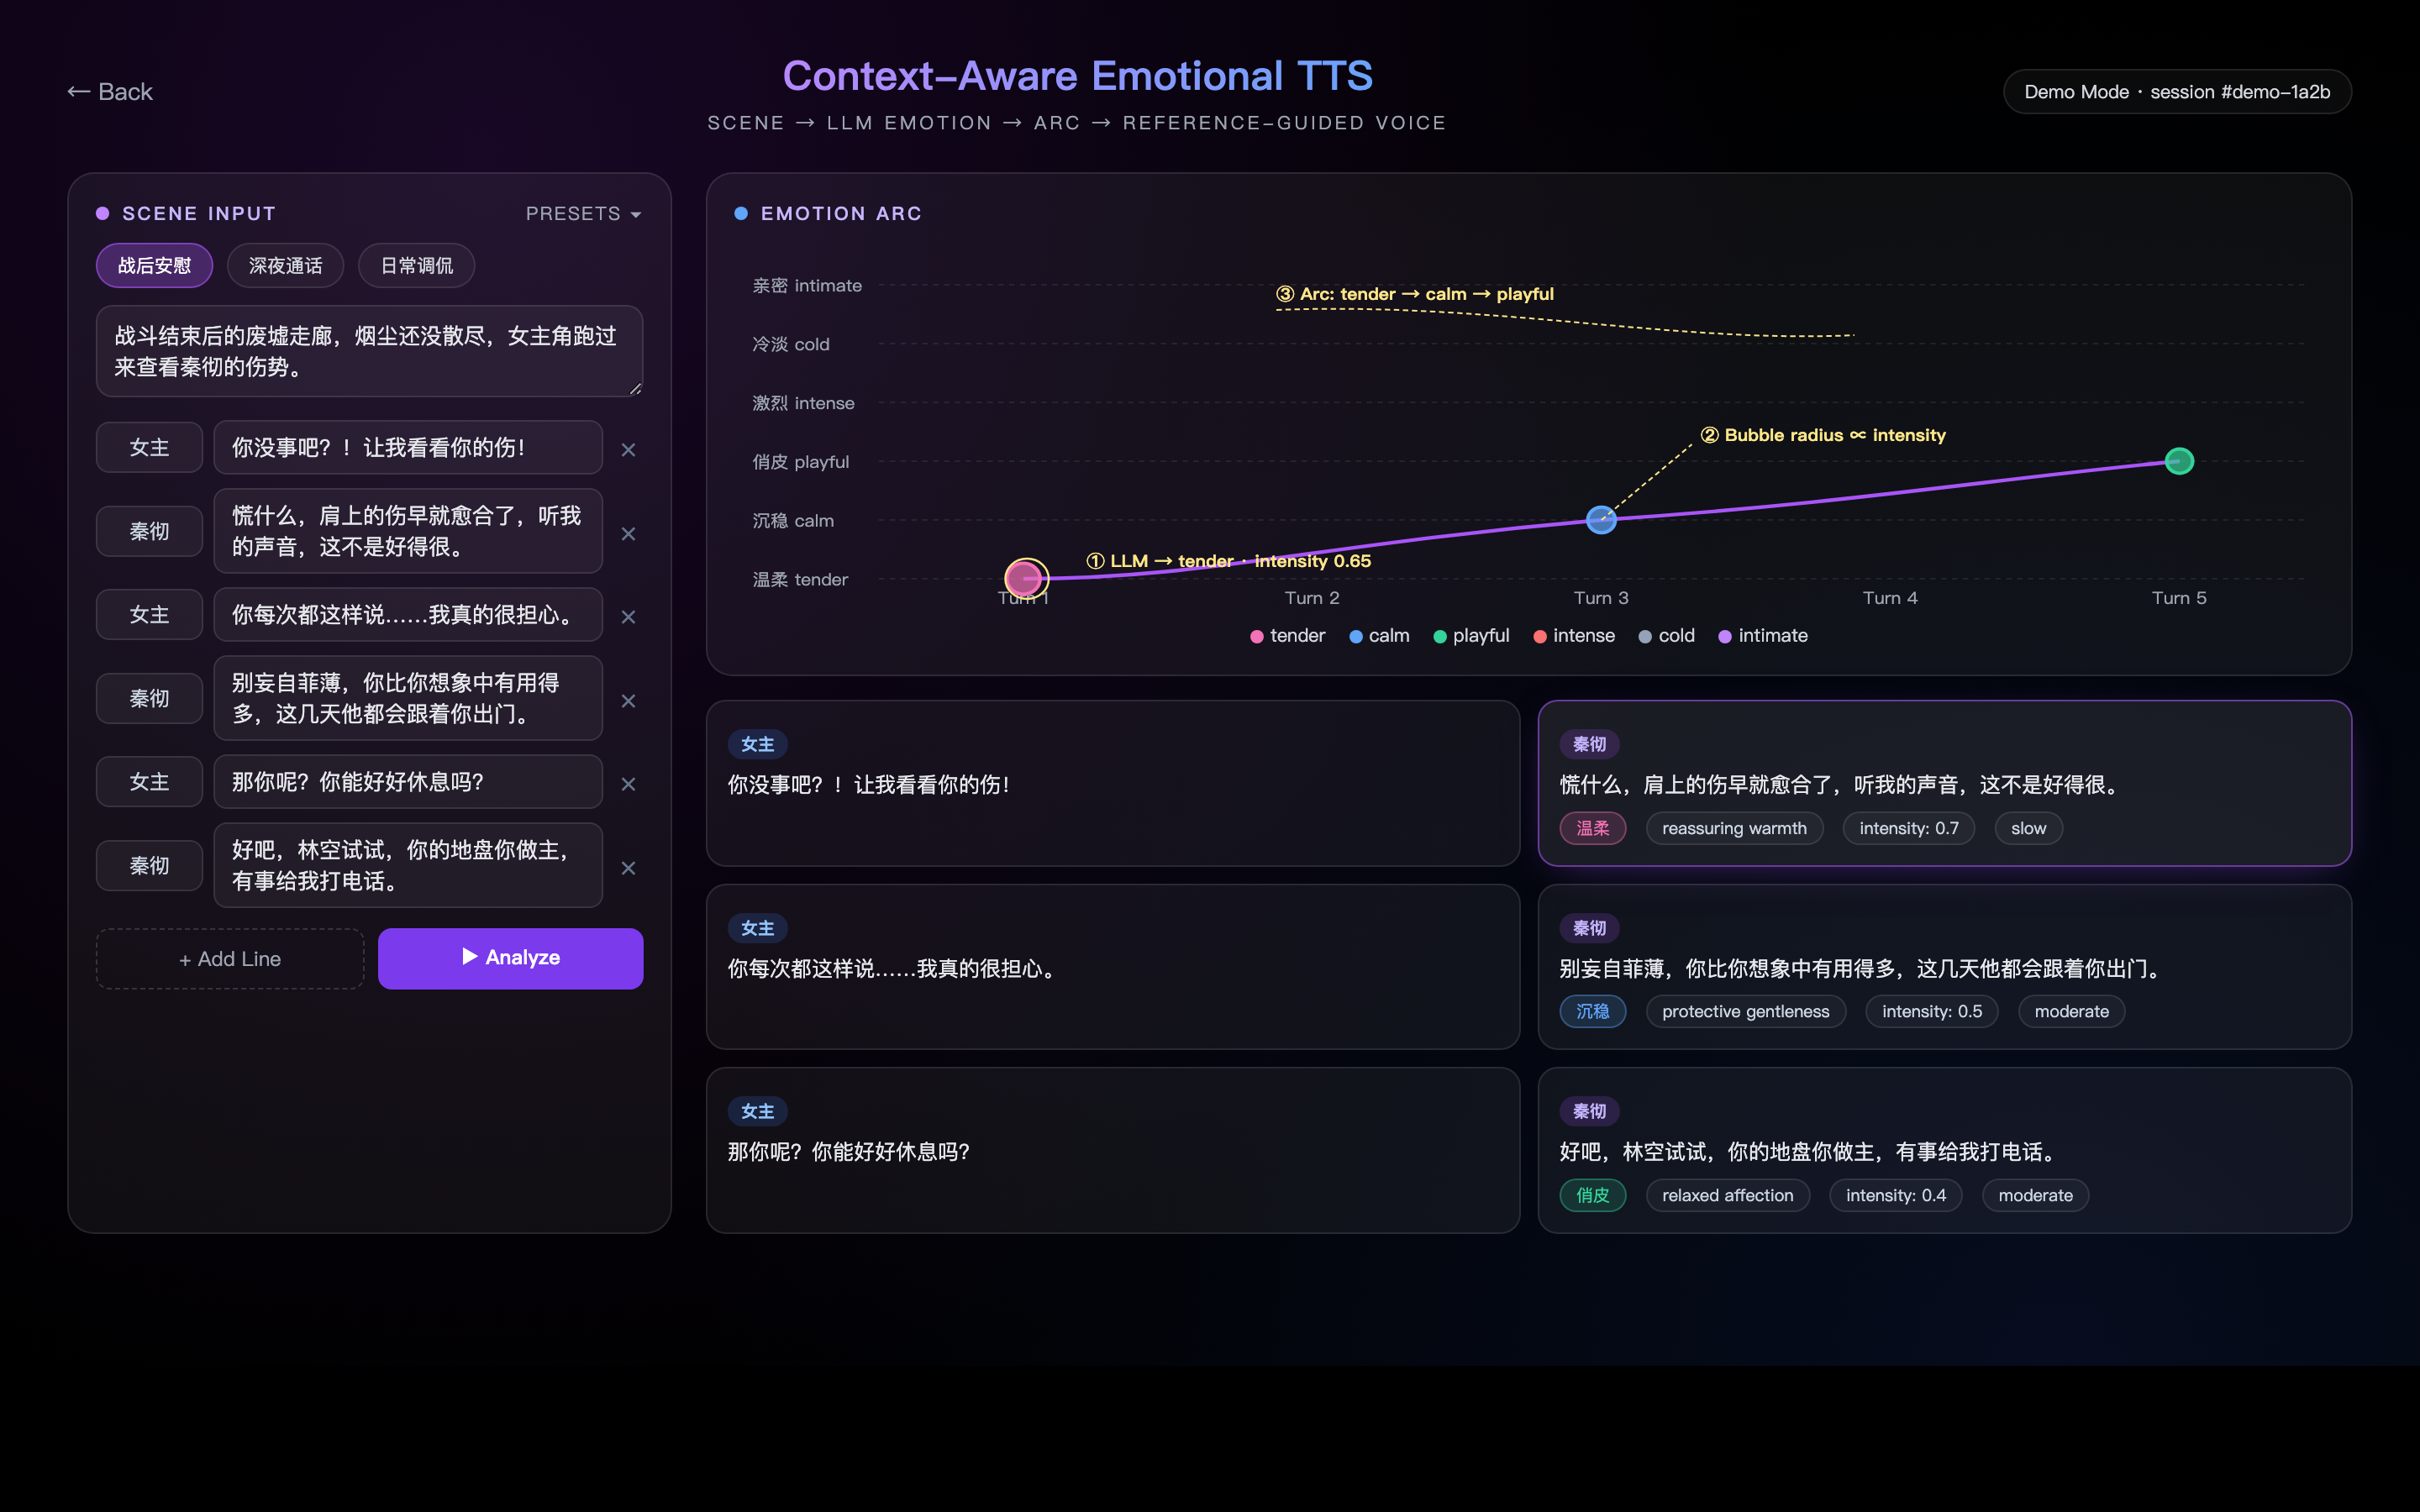
\includegraphics[width=\linewidth]{figs/ui_arc.png}
  \caption{Scene input + Emotion Arc (Demo Mode). \textcircled{\scriptsize 1}~LLM emotion label, \textcircled{\scriptsize 2}~bubble radius $\propto$ intensity, \textcircled{\scriptsize 3}~arc across turns.}
  \label{fig:ui-arc}
\end{subfigure}\hfill
\begin{subfigure}[t]{0.495\linewidth}
  \centering
  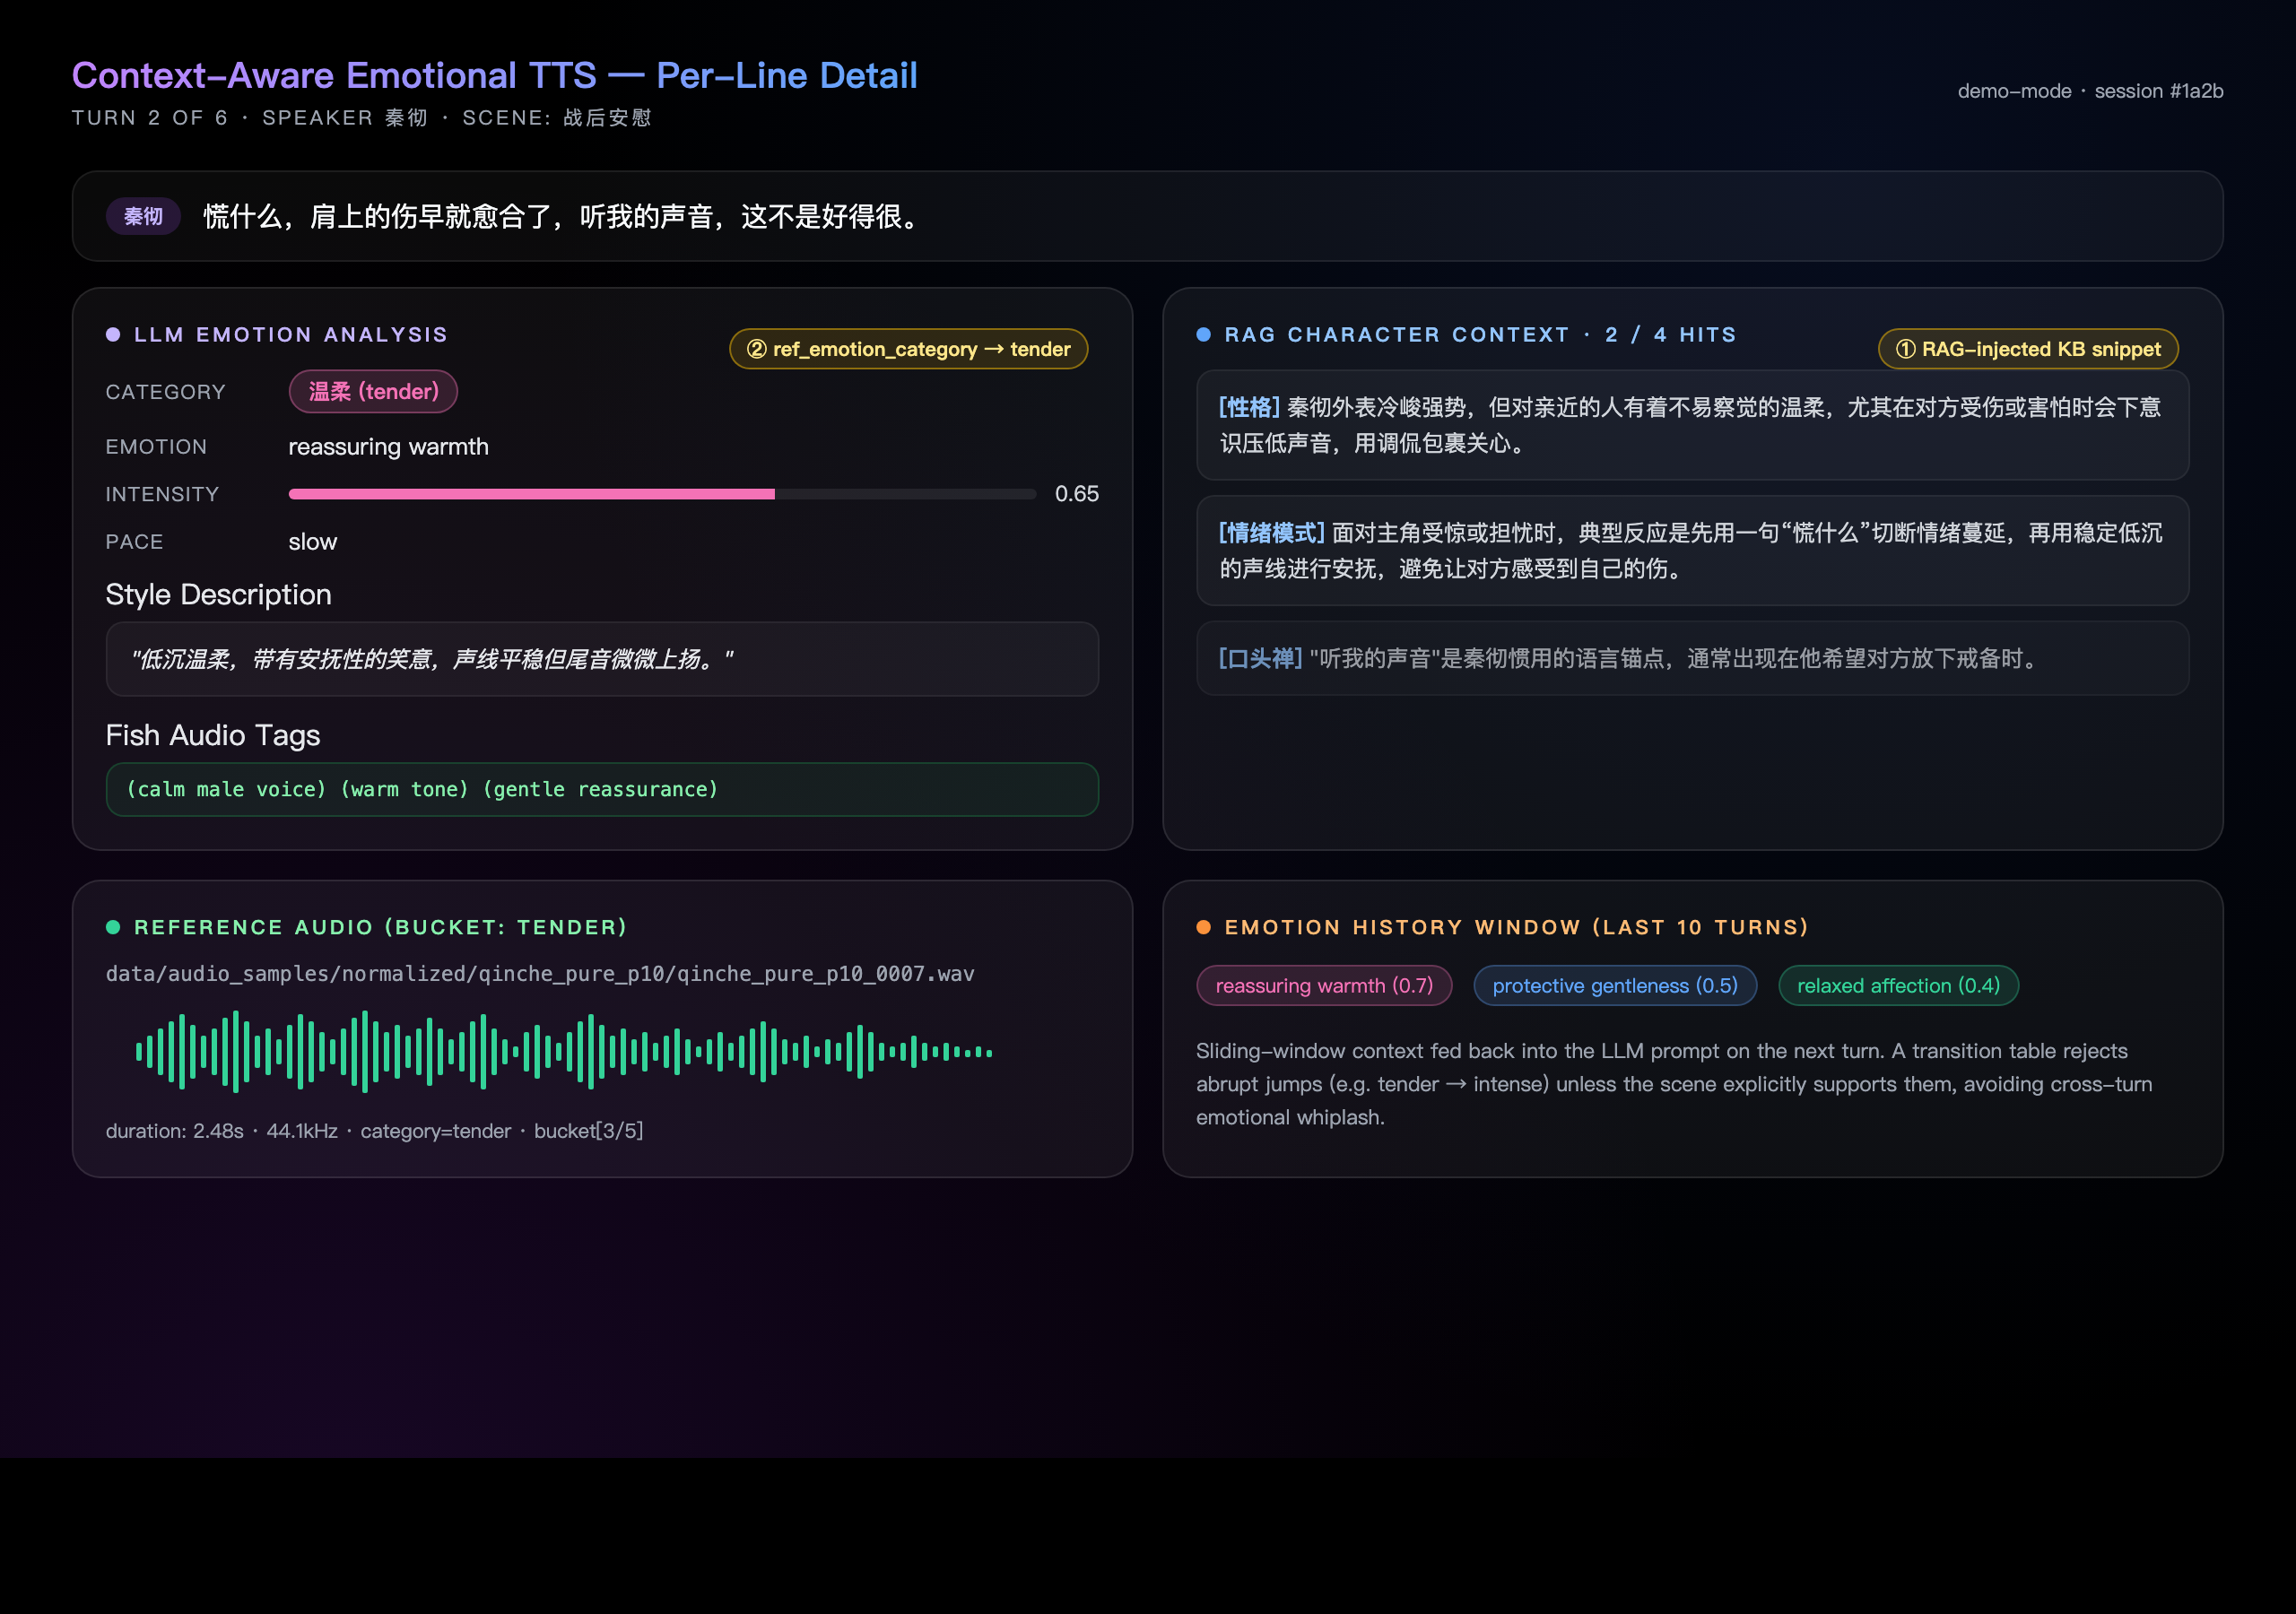
\includegraphics[width=\linewidth]{figs/ui_detail.png}
  \caption{Per-line detail panel: LLM analysis, \textcircled{\scriptsize 1}~RAG-injected KB snippet, picked \textcircled{\scriptsize 2}~\texttt{ref\_emotion\_category}, reference-audio waveform, and 10-turn history.}
  \label{fig:ui-detail}
\end{subfigure}
\caption{\textbf{Frontend visualization of the emotional TTS pipeline} (\texttt{frontend/src/pages/EmotionalTTSPage.tsx}). Both panels are rendered from the same offline \emph{Demo Mode} data, so teammates can iterate on UX without a GPU or an API key.}
\label{fig:ui}
\end{figure}

\begin{figure}[H]
\centering
\includegraphics[width=0.82\linewidth]{figs/emotion_and_phase1.pdf}
\caption{\textbf{(a)}~Distribution of the 30 curated emotion-bucket references (5 per category) distilled from the 664 training clips; the flat distribution is intentional so the dispatcher always has a matching reference regardless of the LLM label. \textbf{(b)}~Phase-1 objective numbers: our Qwen3 SFT~v5~ep3 is tied with Qwen ZS on SIM\_gt (0.689 vs 0.710) but halves WER (4.25\% vs 12.0\%), and dominates Fish~S2~Pro on SIM\_gt at similar WER --- the remaining quality headroom is in \emph{emotion}, not timbre.}
\label{fig:phase1}
\end{figure}

%% ============================================================
\section{Remaining Tasks \& Timeline}\label{sec:remaining}
%% ============================================================
\begin{itemize}
  \item \textbf{Apr 18 -- Apr 24: three-way comparative evaluation.} Run \texttt{src/eval/run\_eval.py} on the 18-sentence set plus 20 new scripted scenes in three conditions: (A) no context, (B) hand-annotated emotions, (C) our LLM context pipeline. Objective metrics: SIM\_gt, SIM\_ref, WER, emotion accuracy via \texttt{emotion2vec}; artifact: updated \texttt{docs/eval\_summary.json}.
  \item \textbf{Apr 25 -- May 1: subjective A/B + MOS.} 10+ evaluators, 20 paired samples, blind 5-point MOS on naturalness + emotional appropriateness; the A/B player is an extension of \texttt{EmotionalTTSPage.tsx} so the UI doubles as the evaluation tool.
  \item \textbf{May 2 -- May 10: final deliverables.} 4--6 page report, 3-min demo video, code freeze. Risks: OpenRouter rate limits (mitigated by a local Qwen2.5 fallback already wired into \texttt{analyzer.py}) and MOS recruitment (course cohort + internal team).
\end{itemize}

\vspace{2pt}
\begin{infobox}
\small
{\sffamily\bfseries\color{primary}Repository \& demo}\par\vspace{2pt}
\begin{tabular}{@{}>{\sffamily\bfseries\color{primary}}p{0.16\linewidth}@{\hspace{0.4em}}p{0.80\linewidth}@{}}
Source        & \url{https://github.com/darkknightyh/qinche-emotional-tts}\quad{\footnotesize\color{mutedtext}\itshape(placeholder --- final URL to be replaced before submission)} \\
Live demo     & \url{https://qinche.darkdark.me}\quad{\footnotesize\color{mutedtext}Phase-1 cloner live; Phase-2 page on \texttt{/emotional-tts} once deployed} \\
Phase-1 report & \texttt{docs/report/report.pdf} \\
Proposal      & \texttt{docs/proposal/proposal.md} \\
\end{tabular}
\end{infobox}

\end{document}
